\documentclass[../../main/main.tex]{subfiles}
\graphicspath{{./figures/}}

\dominitoc
\faketableofcontents

\makeatletter
\renewcommand{\@chapapp}{\'Electrocin\'etique -- chapitre}
\makeatother

% \toggletrue{student}
% \HideSolutionstrue
\toggletrue{corrige}
\renewcommand{\mycol}{black}
% \renewcommand{\mycol}{gray}

\begin{document}
\setcounter{chapter}{1}

\chapter{R\'esistances et sources}

\vfill

\begin{prgm}
	\begin{tcb}*(ror)"know"{Savoirs}
		\begin{itemize}[label=$\diamond$, leftmargin=10pt]
			\item Connaître les relations entre l'intensité et la tension.
			      % \item Citer des ordres de grandeurs des composants R, L, C.
			\item Exprimer la puissance dissipée par effet \textsc{Joule} dans une
			      résistance.
			      % \item Exprimer l'énergie stockée dans un condensateur ou une bobine.
		\end{itemize}
	\end{tcb}

	\begin{tcb}*(ror)"how"{Savoir-faire}
		\begin{itemize}[label=$\diamond$, leftmargin=10pt]
			\item Remplacer une association série ou parallèle de deux
			      résistances par une résistance équivalente.
			\item Établir et exploiter les relations des diviseurs de
			      tension ou de courant.
			\item Modéliser une source en utilisant la représentation de
			      \textsc{Thévenin}.
			\item Évaluer une résistance d'entrée ou de sortie à
			      l'aide d'une notice ou d'un appareil afin d'appréhender les
			      conséquences de leurs valeurs sur le fonctionnement d'un circuit.
			\item Étudier l'influence des résistances d'entrée ou de
			      sortie sur le signal délivré par un GBF, sur la mesure effectuée par
			      un oscilloscope ou un multimètre.
		\end{itemize}
	\end{tcb}
\end{prgm}

\vfill
\minitoc
\vfill

\newpage

\section{Généralité sur les dipôles}
\subsection{Caractéristique d'un dipôle}
\begin{tcbraster}[raster columns=2, raster equal height=rows]
	\begin{tcb}[label=def:dipcara](defi){Caractéristique}

		On appelle \textbf{caractéristique} d'un dipôle la fonction $I = f(U)$
		(ou $U = g(I)$ selon la convention). Sauf indication contraire, elle est
		déterminée \textbf{en régime continu}.

		\tcbsubtitle{\fatbox{Cas particuliers}}
		\begin{itemize}
			\item \psw{
				      \textbf{Court-circuit} (fil branché aux bornes) $\Ra $
				      $U = 0$, et ce pour tout $I$.
			      }
			\item \psw{
				      Un dipôle qui n'est
				      \textbf{pas relié à un circuit fermé} a pour intensité $I = 0$.
			      }
		\end{itemize}
	\end{tcb}
	\begin{tcb}[label=exem:dipcara](exem)'r'{Exemple}
		\begin{center}
			\switch{
				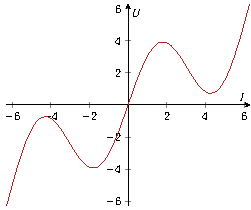
\includegraphics[width=\linewidth, draft=true]{carac_gen}
			}{
				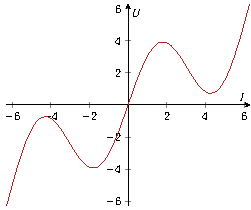
\includegraphics[width=\linewidth]{carac_gen}
			}
		\end{center}
	\end{tcb}
\end{tcbraster}

\subsection{Classification de dipôles}
\begin{tcb}[label=def:actifpassif, tabularx={Y|Y|Y}](defi){Actif ou passif,
			linéaire ou non, symétrique ou non}

	\tcbsubtitle{\fatbox{Passif}}
	\begin{itemize}
		\item \psw{
			      \textbf{Pas} alimenté.
		      }
		\item \psw{
			      \textbf{Passe par (0,0)}.
		      }
		\item \psw{
			      Convention \textbf{récepteur}.
		      }
	\end{itemize}
	&
	\tcbsubtitle{\fatbox{Linéaire}}
	\psw{
		Un dipôle est dit \textbf{linéaire} si sa caractéristique est une
		\textbf{droite}.
	}
	&
	\tcbsubtitle{\fatbox{Symétrique}}
	\psw{
		\textbf{Symétrique} $\Lra$ \textbf{impaire}. \fbox{Symétrique $\Ra$ passif}.
	}
	\\
	\tcbsubtitle{\fatbox{Actif}}
	\begin{itemize}
		\item \psw{
			      \textbf{Est} alimenté.
		      }
		\item \psw{
			      \textbf{Passe pas par (0,0)}.
		      }
		\item \psw{
			      Convention \textbf{générateur}.
		      }
	\end{itemize}
	&
	\tcbsubtitle{\fatbox{Non-linéaire}}
	\psw{
		Un dipôle est dit \textbf{non-linéaire} si sa caractéristique n'est
		\textbf{pas une droite}.
	}
	&
	\tcbsubtitle{\fatbox{Asymétrique}}
	\psw{
		\textbf{Asymétrique} si sa caractéristique n'est \textbf{pas impaire}.
	}
\end{tcb}

\section{Résistance}
\subsection{Définition et schéma}

Lorsqu'un courant circule dans un matériau conducteur, les électrons sont
freinés par les atomes de celui-ci. Cet effet est maximal dans certains dipôles
que l'on appellera des conducteurs ohmiques ou résistors. Par abus de langage,
on désignera le composant par le même nom que la grandeur physique qui le
caractérise~: la résistance.

\begin{tcb}[label=def:resistance, sidebyside](defi){Résistance}
	Une résistance est un dipôle \textbf{récepteur}, dont la caractéristique en
	convention récepteur suit la \textbf{loi d'Ohm}~:
	\psw{
		\[
			\boxed{U=RI}
			\Lra
			\boxed{GU=I}
		\]
	}
	\vspace{-15pt}
	\tcblower
	\tcbsubtitle{\fatbox{Unités}}
	\begin{itemize}
		\item \psw{
			      Résistance en Ohm ($\Omega$) avec $R > 0$.
		      }
		\item \psw{
			      Conductance \fbox{$G=1/R$} en Siemens (S).
		      }
	\end{itemize}
\end{tcb}
\begin{tcbraster}[raster columns=2, raster equal height=rows]
	\begin{tcb}[label=impl:resistance](impl){Puissance}
		En utilisant la caractéristique de la résistance et l'expression de la
		puissance d'un dipôle, on a
		\psw{
			\[
				\boxed{P_{\text{reçue}} = RI^2 = \frac{U^2}{R} = GU^2}
			\]
		}
		Qui est positive. Dans le cas de la résistance, cette puissance est
		entièrement \textbf{dissipée} par effet \textsc{Joule}.
		\begin{center}
			\switch{
				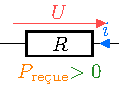
\includegraphics[width=.6\linewidth, draft=true]{resistance}
			}{
				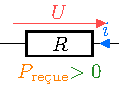
\includegraphics[width=.6\linewidth]{resistance}
			}
		\end{center}
	\end{tcb}
	\begin{tcb}[label=exem:resistance](exem)'r'{Caractéristique}
		\begin{center}
			\switch{
				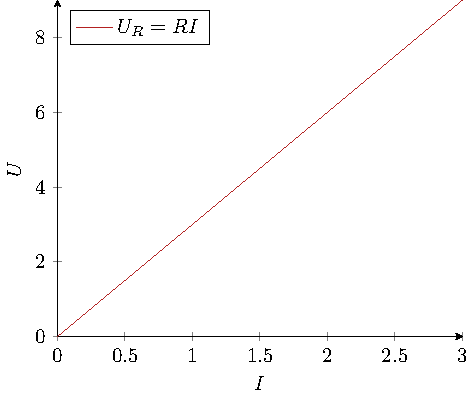
\includegraphics[width=\linewidth, draft=true]{carac_R}
			}{
				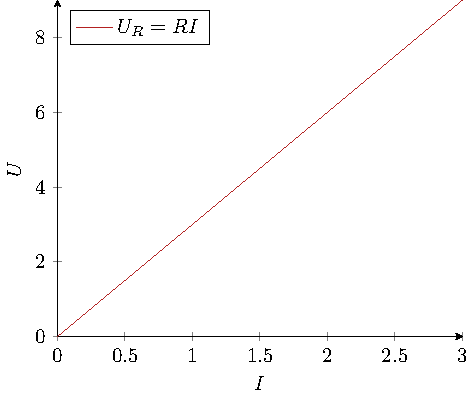
\includegraphics[width=\linewidth]{carac_R}
			}
			\captionof{figure}{Caractéristique d'une résistance.}
		\end{center}
	\end{tcb}
\end{tcbraster}


\subsection{Association de résistances en série}
\begin{tcbraster}[raster columns=2, raster equal height=rows]
	\begin{tcb}[label=prop:rserie](prop){Association en série}
		Deux résistances $R_1$ et $R_2$ en série forment un dipôle équivalent de
		résistance
		\psw{
			\[
				\boxed{R_{\rm eq} = R_1 + R_2}
			\]
		}
		On dit qu'\textbf{en série, les résistances s'ajoutent}.
		\tcblower
		\begin{center}
			\switch{
				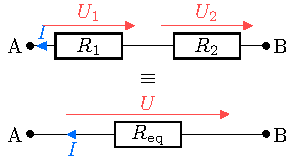
\includegraphics[width=\linewidth, draft=true]{rserie}
			}{
				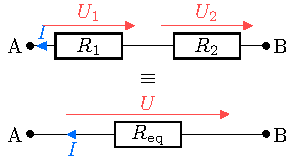
\includegraphics[width=\linewidth]{rserie}
			}
		\end{center}
	\end{tcb}
	\begin{tcb}[label=demo:rserie](demo)'r'{Association en série}
		\psw{
			À partir du schéma précédent, on écrit la loi d'additivité des tensions,
			puis on applique la loi d'Ohm et on factorise~:
			\begin{align*}
				U & = U_1 + U_2    \\
				U & = R_1I + R_2I  \\
				U & = (R_1 + R_2)I
			\end{align*}
			On a bien l'expression d'un unique conducteur ohmique de résistance
			\fbox{$R_{\rm eq} = R_1 + R_2$}.
		}
	\end{tcb}
\end{tcbraster}

\subsection{Association de résistances en parallèle}
\begin{tcbraster}[raster columns=2, raster equal height=rows]
	\begin{tcb}[label=prop:rpara](prop){Association en parallèle}
		Deux résistances $R_1$ et $R_2$ en dérivation forment un dipôle
		équivalent de résistance
		\psw{
			\[
				\boxed{\dfrac{1}{R_{\rm eq}} = \dfrac{1}{R_1} + \dfrac{1}{R_2}}
				\Lra
				\boxed{G_{\rm eq} = G_1+G_2}
			\]
		}
		On dit qu'\textbf{en parallèle, l'inverse des résistances s'ajoutent}.
		\tcblower
		\begin{center}
			\switch{
				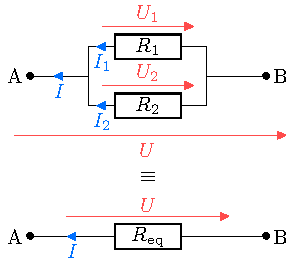
\includegraphics[width=\linewidth, draft=true]{rpara}
			}{
				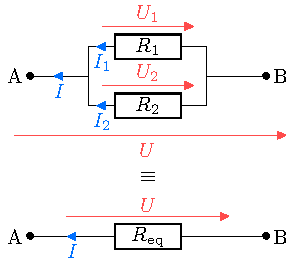
\includegraphics[width=\linewidth]{rpara}
			}
		\end{center}
	\end{tcb}
	\begin{tcb}[label=demo:rpara](demo)'r'{Association en parallèle}
		\psw{
		On applique la loi des nœuds~:
		\[I = I_1+I_2\]
		On utilise ensuite la loi d'Ohm~:
		\[
			I = \frac{U}{R_1} + \frac{U}{R_2}
		\]
		On trouve $R_{\rm eq}$ en exprimant la caractéristique du dipôle
		équivalent sous la forme $I = G_{\rm eq}U$, puis $G_{\rm eq} = 1/R_{\rm
			eq}$, d'où ici
		\[
			I = \left(\dfrac{1}{R_1} + \dfrac{1}{R_2}\right) U
		\]
		On a bien l'expression d'un unique conducteur ohmique de résistance
		\[
			\boxed{\dfrac{1}{R_{\rm eq}} = \dfrac{1}{R_1} + \dfrac{1}{R_2}}
			\Lra
			\boxed{R_{\rm eq} = \frac{R_1R_2}{R_1 + R_2}}
		\]
		}
	\end{tcb}
\end{tcbraster}
\begin{tcb}[sidebyside, lefthand ratio=.4, sidebyside align=top](appl){Exercice
			d'application}

	Exprimer en fonction de $R$ la résistance équivalente entre A et B pour
	l'association ci-dessous.
	\begin{center}
		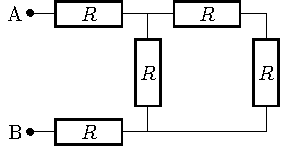
\includegraphics[width=\linewidth]{exer_rasso-plain}
	\end{center}
	\hspace{-15pt}
	\hdashrule[0.5ex]{1.15\linewidth}{.5pt}{1mm}
	\vspace{-15pt}
	\psw{
		\begin{align*}
			R_{\rm eq} & =
			\textcolor{\switch{white}{orange}}{R + R} +
			\textcolor{\switch{white}{brandeisblue}}{R_{\rm eq,2}}  \\ \Lra
			R_{\rm eq} & =
			\textcolor{\switch{white}{orange}}{2R} +
			\textcolor{\switch{white}{brandeisblue}}{
				\frac{
					R\times \textcolor{\switch{white}{ForestGreen}}{R_{\rm eq,1}}
				}{
					R + \textcolor{\switch{white}{ForestGreen}}{R_{\rm eq,1}}
				}
			}
			\\ \Lra
			R_{\rm eq} & =
			2R + \frac{
				R\times\textcolor{\switch{white}{ForestGreen}}{2R}
			}{
				R+\textcolor{\switch{white}{ForestGreen}}{2R}
			}
			\\ \Lra
			R_{\rm eq} & = 2R + \frac{2R^{\cancel{2}}}{3\cancel{R}}
			\\ \Lra
			R_{\rm eq} & = \frac{8R}{3}
		\end{align*}
	}
	\vspace{-15pt}
	\tcblower
	\begin{center}
		\switch{
			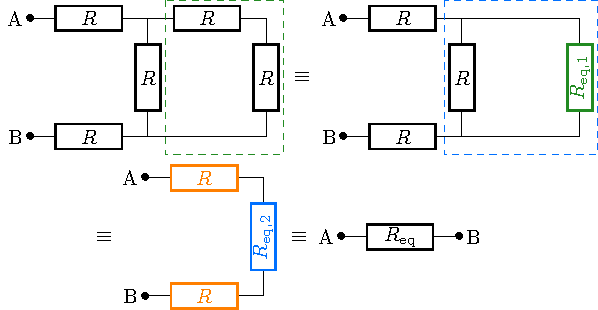
\includegraphics[width=\linewidth, draft=true]{exer_rasso}
		}{
			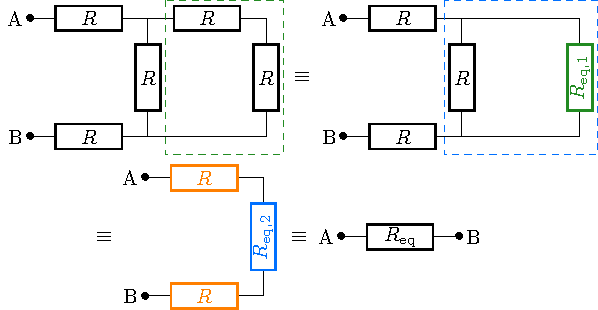
\includegraphics[width=\linewidth]{exer_rasso}
		}
	\end{center}
\end{tcb}

\section{Sources}
\subsection{Sources de tension}

\begin{tcbraster}[raster columns=2, raster equal height=rows]
	\begin{tcb}[label=def:gentens](defi){Générateur idéal de tension}
		\begin{isd}
			Il \textbf{impose une tension}, le courant débité
			est lui imposé par le reste du circuit électrique.
			\tcblower
			Il est dit \textbf{idéal} si la tension imposée est constante quel que
			soit le courant débité.
		\end{isd}
		\begin{center}
			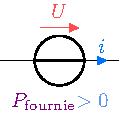
\includegraphics[width=.4\linewidth]{gconvg}
		\end{center}
	\end{tcb}
	\begin{tcb}[label=exem:gentens](exem)'r'{Caractéristique}
		\begin{center}
			\switch{
				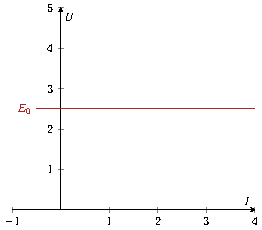
\includegraphics[width=.7\linewidth, draft=true]{carac_tens}
			}{
				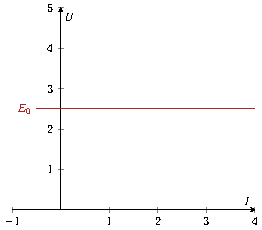
\includegraphics[width=.7\linewidth]{carac_tens}
			}
			\captionof{figure}{Caractéristique d'une tension idéale.}
		\end{center}
	\end{tcb}
\end{tcbraster}

% \subsection{Source réelle de tension}
\begin{tcbraster}[raster columns=2, raster equal height=rows]
	\begin{tcb}[label=def:gentens](defi){Générateur réel de tension}
		\begin{isd}[sidebyside align=top]
			À cause des effets résistifs, la tension imposée et le courant débité sont
			liés~:
			\psw{
				\[\boxed{U = E_0 - ri}\]
			}
			\vspace*{-15pt}
			\tcblower
			On parle de \textbf{générateur de Thévenin}, et
			$E_0$ est la \textbf{force électromotrice}.
		\end{isd}
		\vspace*{-15pt}
		\begin{center}
			% \rotatebox{90}{
			\switch{
				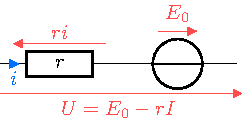
\includegraphics[width=.6\linewidth, draft=true]{thevenin}
			}{
				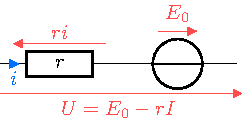
\includegraphics[width=.6\linewidth]{thevenin}
			}
			% }
		\end{center}
	\end{tcb}
	\begin{tcb}[label=exem:gentens](exem)'r'{Caractéristique}
		\begin{center}
			\switch{
				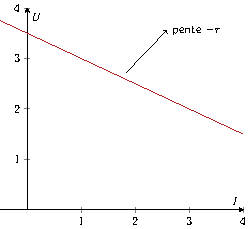
\includegraphics[width=.7\linewidth, draft=true]{carac_thev}
			}{
				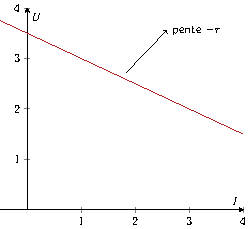
\includegraphics[width=.7\linewidth]{carac_thev}
			}
			\captionof{figure}{Caractéristique d'une tension réelle.}
		\end{center}
	\end{tcb}
\end{tcbraster}

% \vspace{-15pt}
% \subsection{Résistance de sortie}

\begin{tcbraster}[raster columns=2, raster equal height=rows]
	\begin{tcb}[label=prop:rsortie, sidebyside](prop){Résistance de sortie}
		Un générateur réel branché sur une résistance $R$ est
		générateur idéal si
		\[ \boxed{R \gg r}\]
		\tcblower
		\begin{center}
			\switch{
				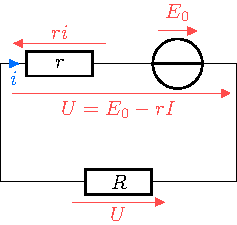
\includegraphics[width=\linewidth, draft=true]{rsortie}
			}{
				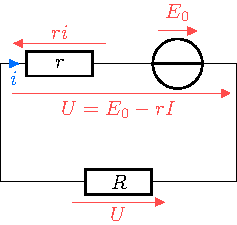
\includegraphics[width=\linewidth]{rsortie}
			}
		\end{center}
	\end{tcb}
	\begin{tcb}[label=demo:rsortie](demo)'r'{Résistance de sortie}
		\psw{
			On applique la formule du pont diviseur de tension pour avoir la tension
			$U$~:
			\[
				U = \frac{R}{R + r}E_0
			\]
			$U \neq E_0$ en général, mais si $R \gg r$ on a tout de même $U \approx
				E_0$.
		}
	\end{tcb}
\end{tcbraster}

\subsection{Sources de courant}

\begin{tcbraster}[raster columns=2, raster equal height=rows]
	\begin{tcb}[label=def:gentens](defi){Générateur idéal de courant}
		\begin{isd}
			Il \textbf{impose un courant}, la tension à ses bornes
			est lui imposé par le reste du circuit électrique.
			\tcblower
			Il est dit \textbf{idéal} si le courant débité est constant quelle que
			soit la tension à ses bornes.
		\end{isd}
		\begin{center}
			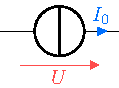
\includegraphics[width=.4\linewidth]{gcourg}
		\end{center}
	\end{tcb}
	\begin{tcb}[label=exem:gentens](exem)'r'{Caractéristique}
		\begin{center}
			\switch{
				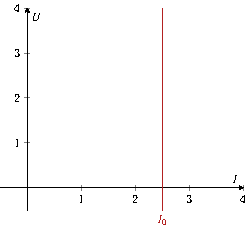
\includegraphics[width=.7\linewidth, draft=true]{carac_cour}
			}{
				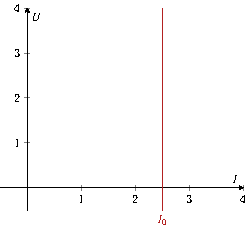
\includegraphics[width=.7\linewidth]{carac_cour}
			}
			\captionof{figure}{Caractéristique d'un courant idéal.}
		\end{center}
	\end{tcb}
\end{tcbraster}

% \subsection{Complément~: source réelle de courant}
\begin{tcbraster}[raster columns=2, raster equal height=rows]
	\begin{tcb}[label=def:gencour, sidebyside](defi){Générateur réel de courant}

		À cause des effets résistifs, on utilise le \textbf{générateur de Norton}.
		\psw{
			\[
				\boxed{I = I_0 - \frac{U}{r_N}}
			\]
		}
		\tcblower
		\begin{center}
			\switch{
				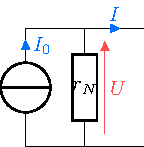
\includegraphics[width=\linewidth, draft=true]{norton}
			}{
				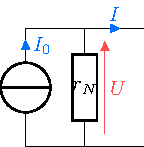
\includegraphics[width=\linewidth]{norton}
			}
		\end{center}
	\end{tcb}
	\begin{tcb}[label=exem:gentens](exem)'r'{Caractéristique}
		\begin{center}
			\switch{
				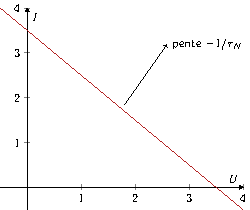
\includegraphics[width=.7\linewidth, draft=true]{carac_nort}
			}{
				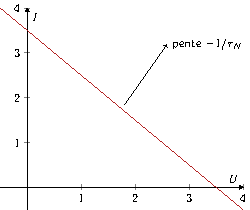
\includegraphics[width=.7\linewidth]{carac_nort}
			}
			\captionof{figure}{Caractéristique d'un courant réel.}
		\end{center}
	\end{tcb}
\end{tcbraster}

% \subsection{Résistance de sortie}

\begin{tcbraster}[raster columns=2, raster equal height=rows]
	\begin{tcb}[label=prop:rsortie, sidebyside](prop){Résistance de sortie}
		Un générateur réel branché sur une résistance $R$ est
		générateur idéal si
		\[ \boxed{R \ll r_N}\]
		\tcblower
		\begin{center}
			\switch{
				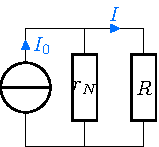
\includegraphics[width=\linewidth, draft=true]{rsortie_intens}
			}{
				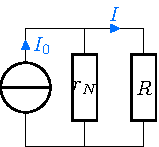
\includegraphics[width=\linewidth]{rsortie_intens}
			}
		\end{center}
	\end{tcb}
	\begin{tcb}[label=demo:rsortie](demo)'r'{Résistance de sortie}
		\psw{
			On applique la formule du pont diviseur de courant pour avoir le courant
			$I$~:
			\[ I = \frac{r_N}{r_N + R}I\]
			$I \neq I_0$ en général, mais si $R \ll r_N$ on a tout de même $I \approx
				I_0$.
		}
	\end{tcb}
\end{tcbraster}

\section{Les ponts diviseurs}

Les ponts diviseurs sont des relations permettant de trouver des courants ou des
tensions dans certains cas particuliers, sans repasser par l'écriture des lois
des nœuds, des mailles et d'Ohm.

\subsection{Pont diviseur de tension}

\begin{tcbraster}[raster columns=2, raster equal height=rows]
	\begin{tcb}[label=prop:divtens, sidebyside](prop){Pont diviseur de tension}
		$U$, $R_1$ et $R_2$ sont connus. On
		cherche $U_1$ ou $U_2$. On a
		\psw{
		\[
			\boxed{U_k = \frac{R_k}{R_1+R_2}U_{\rm brch}}
		\]
		}
		et avec $R_{\rm brch}$ la résistance de toute la branche, on généralise en
		\psw{
		\[
			\boxed{U_k = \frac{R_k}{R_{\rm brch}}U_{\rm brch}}
		\]
		}
		\tcblower
		\begin{center}
			\switch{
				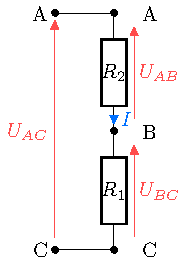
\includegraphics[width=\linewidth, draft=true]{divis_tension}
			}{
				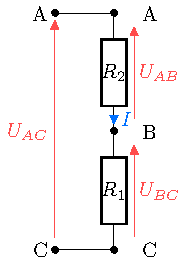
\includegraphics[width=\linewidth]{divis_tension}
			}
		\end{center}
	\end{tcb}
	\begin{tcb}[label=demo:divtens](demo)'r'{Pont diviseur de tension}
		\psw{
		Avec une loi des mailles et la loi d'Ohm pour les résistances, on trouve
		\[
			I = \frac{U_{\rm brch}}{R_1+R_2}
		\]
		En réappliquant la loi d'Ohm pour $R_2$ par exemple, on trouve
		\[
			U_{1} = R_1I = \frac{R_1}{R_1+R_2}U_{\rm brch}
		\]
		Le calcul est tout à fait similaire pour le cas avec plus de résistances
		dans la branche.
		}
	\end{tcb}
\end{tcbraster}

\subsection{Pont diviseur de courant}

\begin{tcbraster}[raster columns=2, raster equal height=rows]
	\begin{tcb}[label=prop:divcour](prop){Pont diviseur de courant}
		$I$, $R_1$ et $R_2$ sont connus. On
		cherche $I_1$ ou $I_2$. On a
		\psw{
		\[
			\boxed{I_k = \frac{G_k}{G_1+G_2}I_{\rm parr}}
			% \Lra
			%    \boxed{I_{\fbox{2}} = \frac{R_{\fbox{1}}}{R_1+R_2}I}
		\]
		}
		Avec $R_{\rm parr}$ la résistance équivalente entre $A$ et $B$, ceci se
		généralise en
		\psw{
		\[
			\boxed{I_k = \frac{G_k}{G_{\rm parr}}I_{\rm parr}}
			\Lra
			\boxed{I_k = \frac{R_{\rm parr}}{R_k}I_{\rm parr}}
		\]
		}
		\tcblower
		\begin{center}
			\switch{
				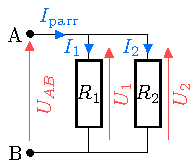
\includegraphics[width=.6\linewidth, draft=true]{divis_courant}
			}{
				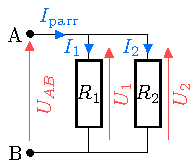
\includegraphics[width=.6\linewidth]{divis_courant}
			}
		\end{center}
	\end{tcb}
	\begin{tcb}[label=demo:divcour](demo)'r'{Pont diviseur de courant}
		\psw{
		Avec la loi des nœuds, on a
		\[I_{\rm parr} = I_1 + I_2\]
		Avec la loi d'Ohm pour les résistances et par égalité des tensions dû au
		montage parallèle, on a
		\[
			I_{\rm parr} =
			\frac{U}{R_1} + \frac{U}{R_2} =
			\frac{U}{R_{\rm eq}} = G_{\rm eq}U
		\]
		D'où, pour $I_1$ par exemple,
		\[
			I_1 = \frac{U}{R_1} = \frac{R_{\rm eq}}{R_1}I_{\rm parr}
		\]
		ou
		\[
			I_1 = G_1 U = \frac{G_1}{G_{\rm eq}}I_{\rm parr}
		\]
		Le calcul est tout à fait similaire pour le cas avec plus de résistances
		en parallèle.
		}
	\end{tcb}
\end{tcbraster}

\subsection{Entraînements}
Donner les expressions de $U_1$, $U_2$, $U_3$ et $U_4$ en fonction de $E$
pour les schémas suivants.
\begin{tcb}[tabularx={Y|Y|Y|Y}](appl){Application~: pont diviseur de tension}
	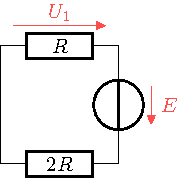
\includegraphics[scale=1]{pdt_a-plain}
	\vspace{12pt}
	% \hdashrule[0.5ex]{1.15\textwidth}{.5pt}{1mm}
	&
	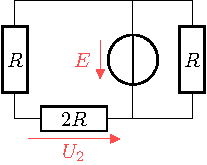
\includegraphics[scale=1]{pdt_b-plain}
	&
	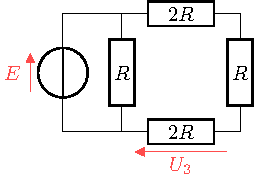
\includegraphics[scale=1]{pdt_c-plain}
	&
	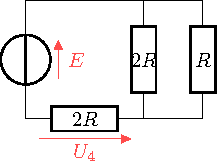
\includegraphics[scale=1]{pdt_d-plain}
	\\
	\begin{center}
		\switch{
			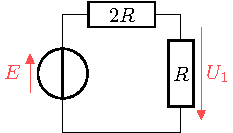
\includegraphics[width=\linewidth, draft=true]{pdt_a}
		}{
			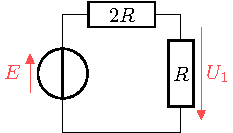
\includegraphics[width=\linewidth]{pdt_a}
		}
	\end{center}
	\psw{
		On a directement
		\[
			\boxed{U_1 = - \frac{1}{3}E}
		\]
	}
	&
	\begin{center}
		\switch{
			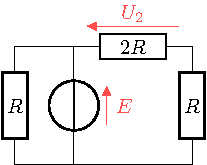
\includegraphics[width=\linewidth, draft=true]{pdt_b}
		}{
			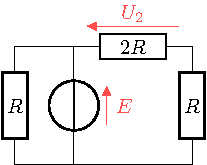
\includegraphics[width=\linewidth]{pdt_b}
		}
	\end{center}
	\psw{
		Avec la rotation du schéma, on voit facilement que
		\[
			\boxed{U_2 = \frac{2}{3}E}
		\]
	}
	&
	\begin{center}
		\switch{
			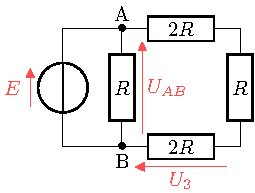
\includegraphics[width=\linewidth, draft=true]{pdt_c}
		}{
			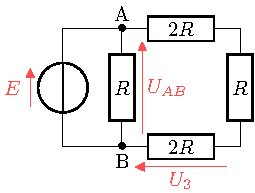
\includegraphics[width=\linewidth]{pdt_c}
		}
	\end{center}
	\psw{
		Ici, on remarque que $U_{AB} = E$. Ainsi
		\[
			\boxed{U_3 = - \frac{2}{5}E}
		\]
	}
	&
	\begin{center}
		\switch{
			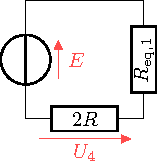
\includegraphics[width=\linewidth, draft=true]{pdt_d}
		}{
			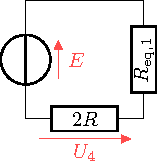
\includegraphics[width=\linewidth]{pdt_d}
		}
	\end{center}
	\psw{
		$R_{\rm eq,1} =\DS \frac{2R^{\cancel{2}}}{3\cancel{R}} = \frac{2R}{3}$,
		d'où
		\[
			\boxed{U_4 = \frac{3}{4}E}
		\]
	}
\end{tcb}

\begin{tcb}[breakable](appl){Application~: pont diviseur de courant}
	\vspace{-10pt}
	\begin{isd}[lefthand ratio=.3]
		Exprimer $I$ selon $I_0$.
		\begin{center}
			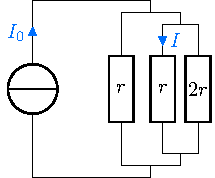
\includegraphics[scale=1]{divcour_last-plain}
		\end{center}
		\tcblower
		\begin{center}
			\switch{
				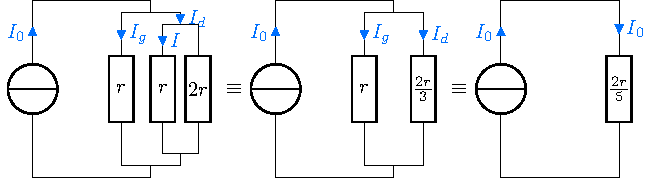
\includegraphics[width=\linewidth, draft=true]{divcour_last-a}
			}{
				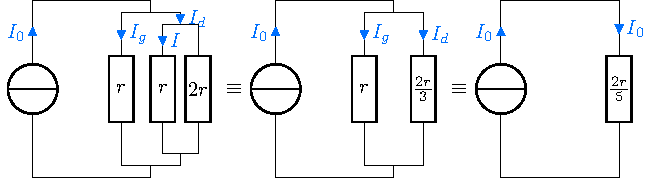
\includegraphics[width=\linewidth]{divcour_last-a}
			}
		\end{center}
	\end{isd}
	\tcblower
	\begin{isd}
		\psw{
			En premier lieu,
			\[ I = \frac{\frac{2r}{3}}{r}I_d = \frac{2}{3}I_d\]
			Ensuite,
			\[ I_d = \frac{ \frac{2r}{5}}{ \frac{2r}{3}}I_0 = \frac{3}{5}I_0\]
		}
		\vspace{-15pt}
		\tcblower
		\psw{
			Ainsi,
			\[ \boxed{I = \frac{2}{5}I_0}\]
		}
	\end{isd}
\end{tcb}

\begin{tcb}*[label=impo:ponts](ror)"bomb"{Utilisation des
	ponts}
	\textbf{Attention} aux conditions d'application de ces formules~: résistances
	\textbf{en série} pour le pont diviseur de \textbf{tension}, et en
	\textbf{parallèle} pour le pont diviseur de \textbf{courant}.
	\smallbreak
	Si non, simplifier le circuit pour se ramener à cette forme. Vérifier
	également \textbf{le sens d'orientation des tensions et intensités}.
\end{tcb}
\vspace{-10pt}
\end{document}
